%-------------------------------------------------------------------
\chapter{Results}
\label{ch:results}
%-------------------------------------------------------------------

\epigraph{\enquote{All models are wrong, but some are useful.}}{\emph{George Box}}

This chapter shows and discusses the results obtained in the thesis.
%In section \ref{sec:experiments} the experimental setting is described and numerical results are reported.
%In section

\section{Experiments}
\label{sec:experiments}

\paragraph{Architecture.}
A neural network model was trained to predict \textit{metric} depth values on image patches.
The neural architecture used is the one from~\cite{Eigen}, with some modification.
Instead of treating it as a two-stage architecture with a component estimating a coarse depth map and another one refining it, it was treated as an end-to-end method.
The network is illustrated in figure~\ref{fig:Eigen}, its backbone is a pretrained AlexNet.
The input image normalization was also modified.
The normalization applied shifts image input values from $[0, 1]$ to $[-1, 1]$.
Finally, an adaptive average pooling layer reduces the deeper feature map of the convolutional part of AlexNet to a feature vector of size 4096.

This model has to be considered a toy model since it is based on the first deep learning architecture ever used for DE (2014).
As later graphs will show, its learning capabilities are limited.

\paragraph{Training.}
The dataset used is KITTI~\cite{KITTI} with the Eigen split, that is the subdivision of the KITTI dataset into train, validation and test subsets originally used by Eigen~et~al. in~\cite{Eigen} and used as a benchmark from there on.
Depth maps are built directly from 3D point clouds, a simplification was performed in this phase to make the code signficantly faster.
This simplification introduces inaccuracies.
But, since training the model like Eigen~et~al. showed only little degradation in metric scores (attributable also the changing on the architectural side), the modification was kept.

The model obtained as input image patches of size fixed to $150 \times 150$.
From each image a batch of 8 patches was extracted.
Two extraction methods were tried: random sampling patches and sampling patches centered in some detected corner.
Patches were further processed before prediction.
It was experimented with geometrical correction of distorsions introduced by the camera far from its principal point.
So experiments were performed either with warping or without it.
After this optional transformation, three options were tried: leave the patch as it is, radially blurring it, uniformly blurring it.

In total there are three options: sampling strategy (random vs corner), patch warping (warp vs no warp), blurring (no blur vs radial blur vs uniform blur).
These result in 12 experiments.

Each experiment consisted in a training of 4 epochs and a stochastic gradient descent optimizer with learning rate 0.0001 and momentum 0.9.
An L1 regularization to the network weights (multiplied by 0.01) was applied for making the algorithm more numerically stable.

The loss function was common to each experiment and is a radially weighted scale invariant loss.
It is a modification of the loss from Eigen~et~al.~\cite{Eigen}.
Their loss is defined in section~\ref{sec:regression_methods}.
Each pixel contribution to the loss is weighted with a gaussian density function with $\sigma = (h + w) / 2$ evaluated in the distance of the pixel from the center of the patch.

\paragraph{Validation.}
Figures \ref{fig:validation} and \ref{fig:Wvalidation} show metrics measured during validation phase.
Both the metrics discussed in section~\ref{sec:metrics} and defined in table~\ref{t:metrics} and their weighted counterparts are shown.
It can be observed that validation performance saturates and sometimes also degrades on the fourth epoch.
This shows that the model learning capabilities are fairly limited as it quickly stops improving itself.
This was expected since the model is old and has known limitations like the fully-connected layers used for up-sampling the feature maps to a depth prediction.
While fully-connected layers proved successful in various tasks, other solutions showed to be more useful in computer vision, as the history of this field proves.

\begin{figure}
    \begin{adjustwidth}{-0.2\textwidth}{-0.2\textwidth}
    \centering
        \begin{subfigure}{0.6\textwidth}
            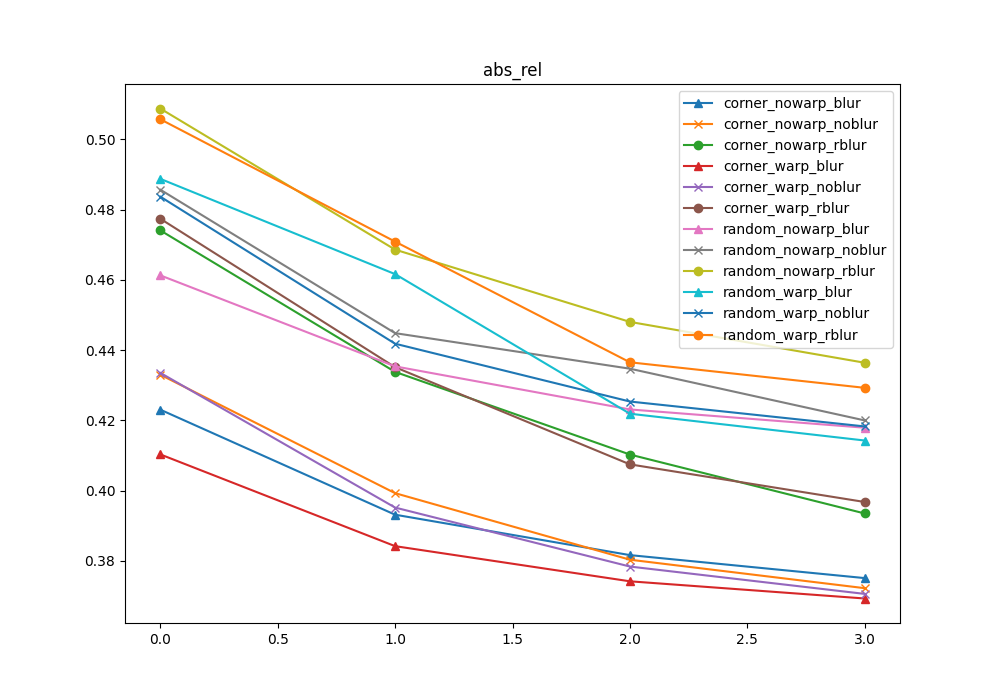
\includegraphics[width=\textwidth]{figs/abs_rel}
        \end{subfigure}
        \hspace{0cm}
        \begin{subfigure}{0.6\textwidth}
            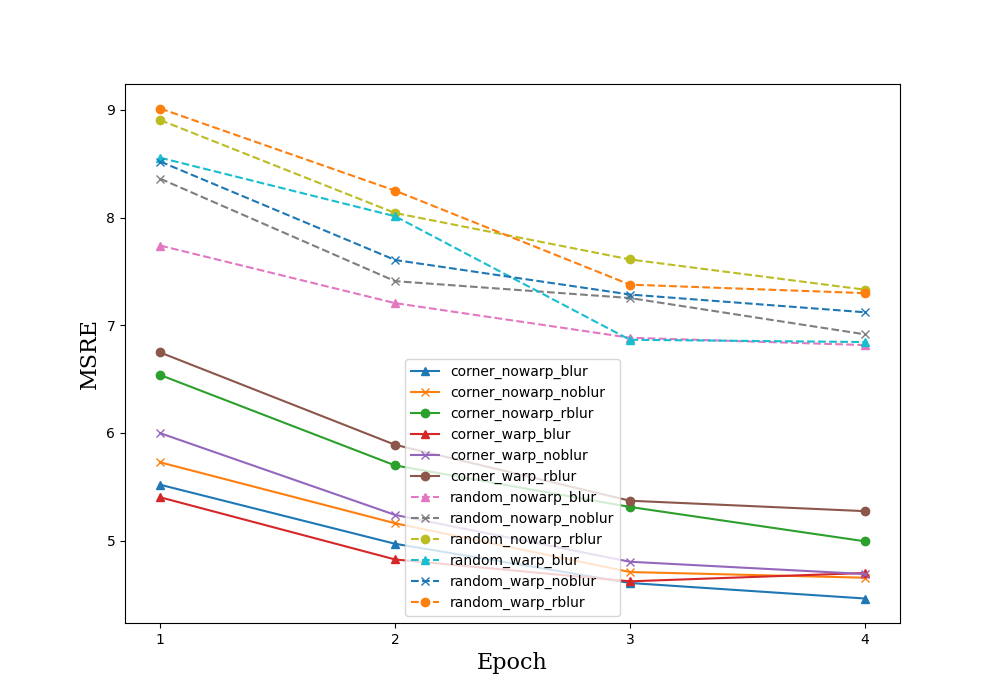
\includegraphics[width=\textwidth]{figs/sq_rel}
        \end{subfigure}
        \hspace{0cm}

        \begin{subfigure}{0.6\textwidth}
            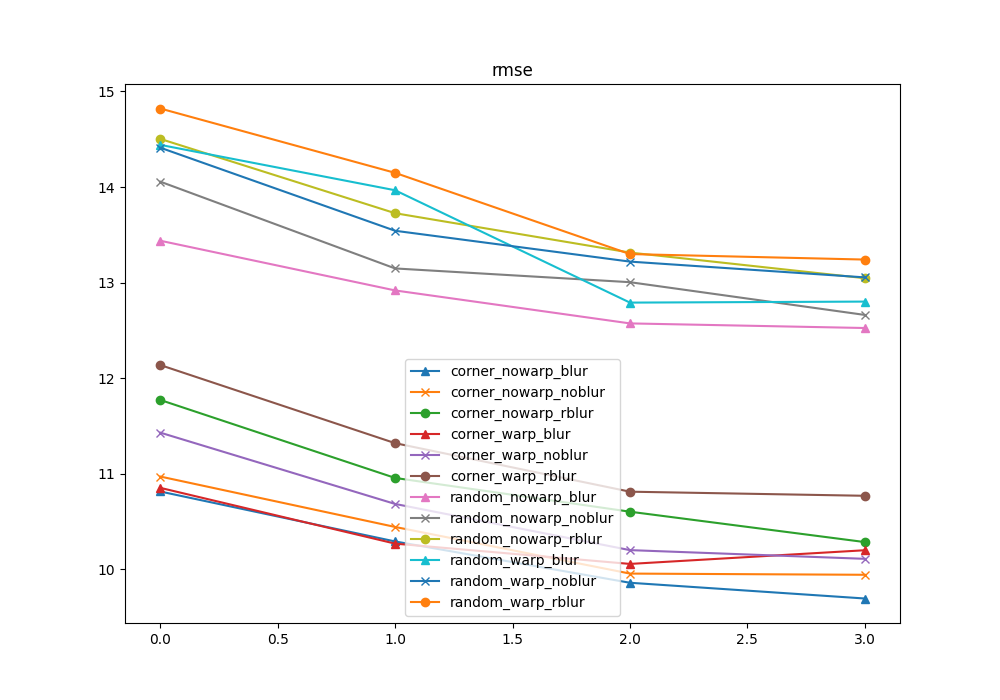
\includegraphics[width=\textwidth]{figs/rmse}
        \end{subfigure}
        \hspace{0cm}
        \begin{subfigure}{0.6\textwidth}
            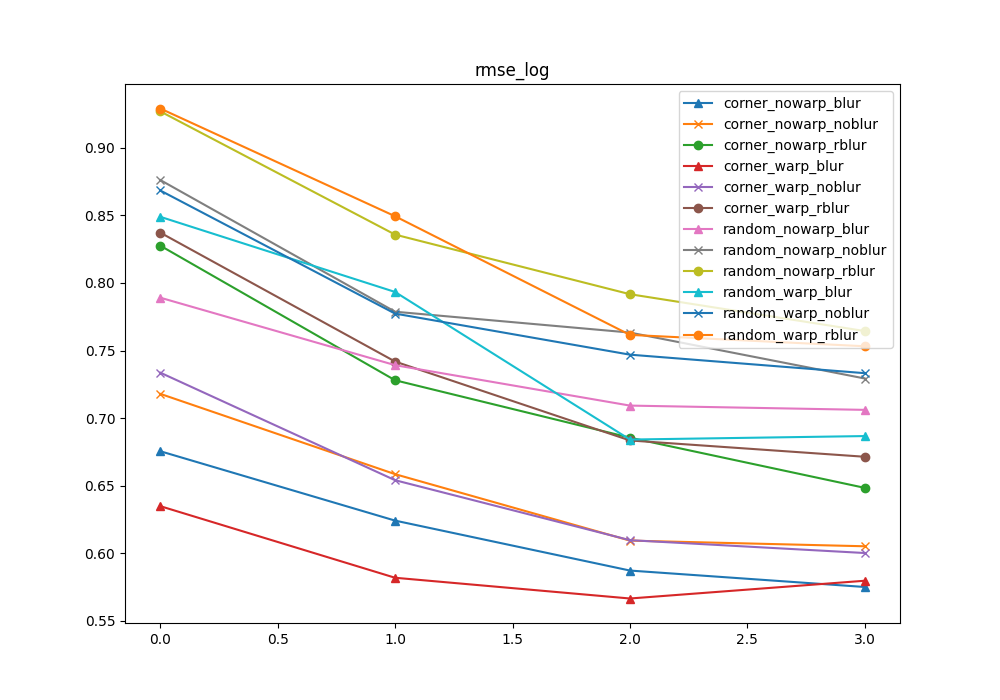
\includegraphics[width=\textwidth]{figs/rmse_log}
        \end{subfigure}
        \hspace{0cm}
        \begin{subfigure}{0.6\textwidth}
            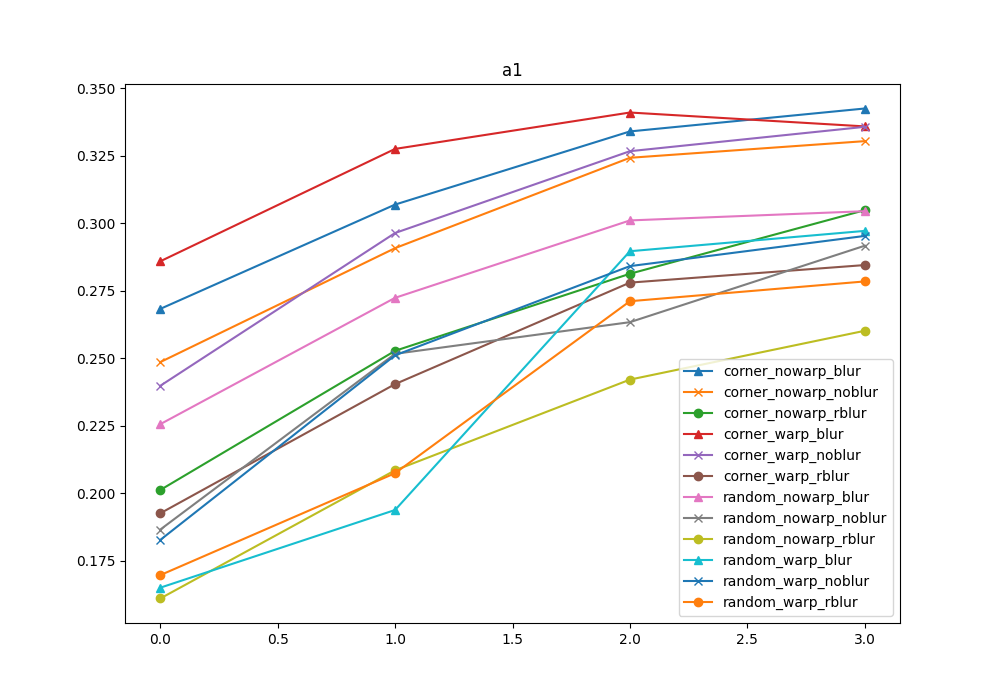
\includegraphics[width=\textwidth]{figs/a1}
        \end{subfigure}
        \hspace{0cm}
        \begin{subfigure}{0.6\textwidth}
            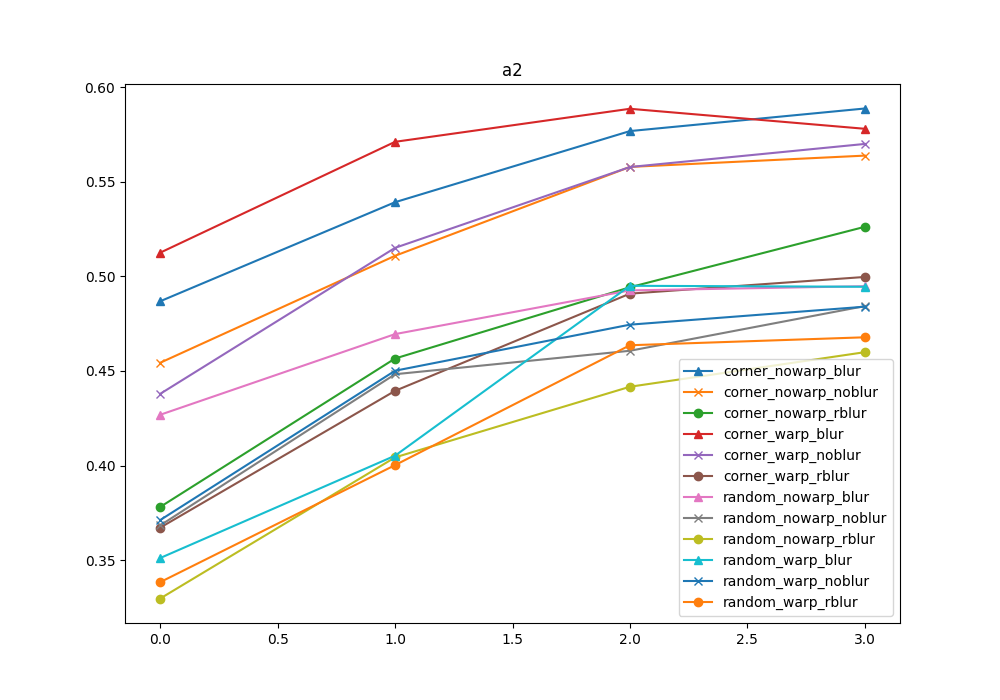
\includegraphics[width=\textwidth]{figs/a2}
        \end{subfigure}
        \hspace{0cm}

        \begin{subfigure}{0.6\textwidth}
            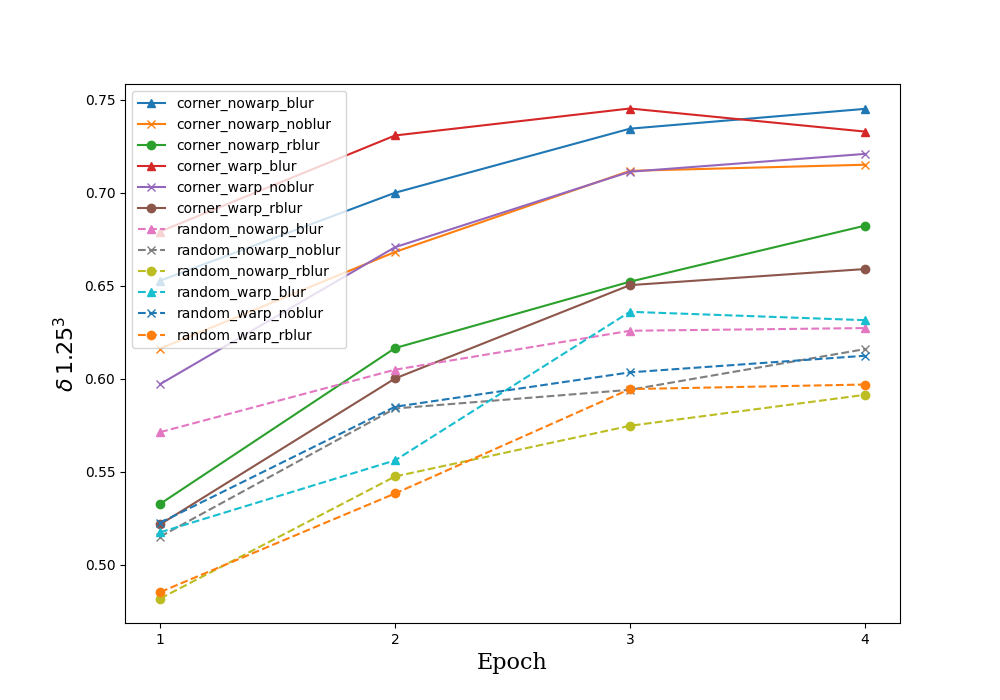
\includegraphics[width=\textwidth]{figs/a3}
        \end{subfigure}
    \end{adjustwidth}
    \caption{
        Non-weighted metrics computed during the validation phase.
        \label{fig:validation}
    }
\end{figure}

\begin{figure}
    \begin{adjustwidth}{-0.2\textwidth}{-0.2\textwidth}
    \centering
        \begin{subfigure}{0.6\textwidth}
            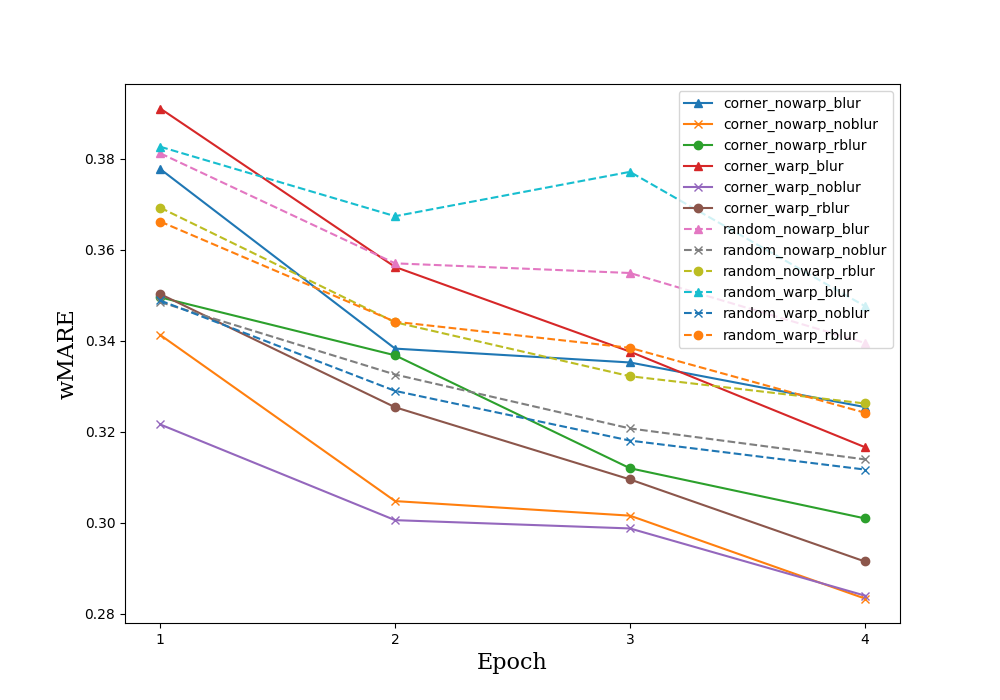
\includegraphics[width=\textwidth]{figs/wabs_rel}
        \end{subfigure}
        \hspace{0cm}
        \begin{subfigure}{0.6\textwidth}
            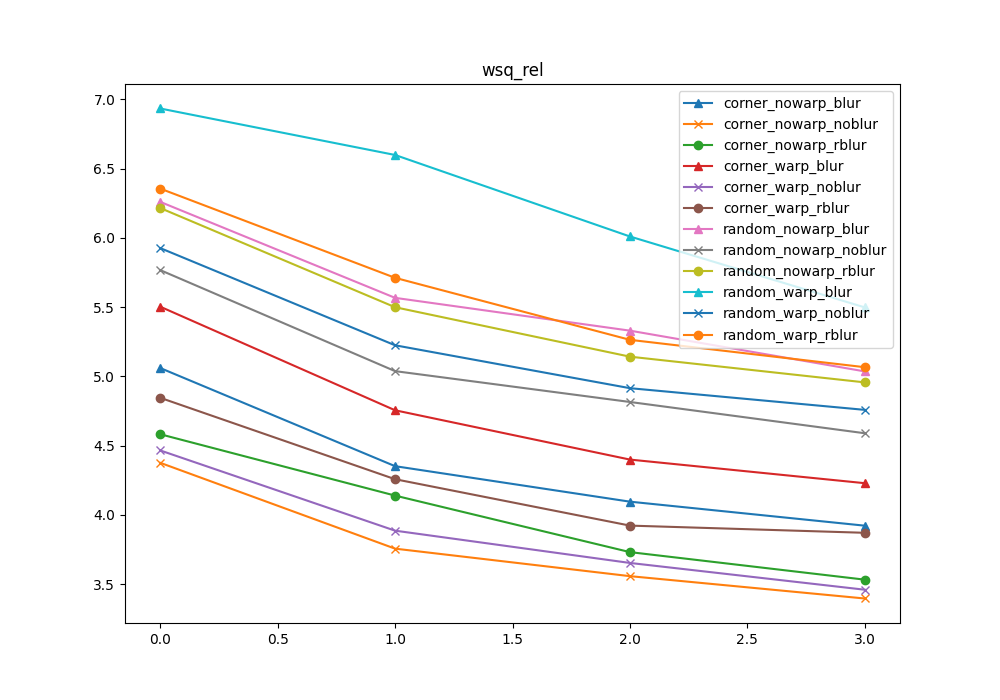
\includegraphics[width=\textwidth]{figs/wsq_rel}
        \end{subfigure}
        \hspace{0cm}

        \begin{subfigure}{0.6\textwidth}
            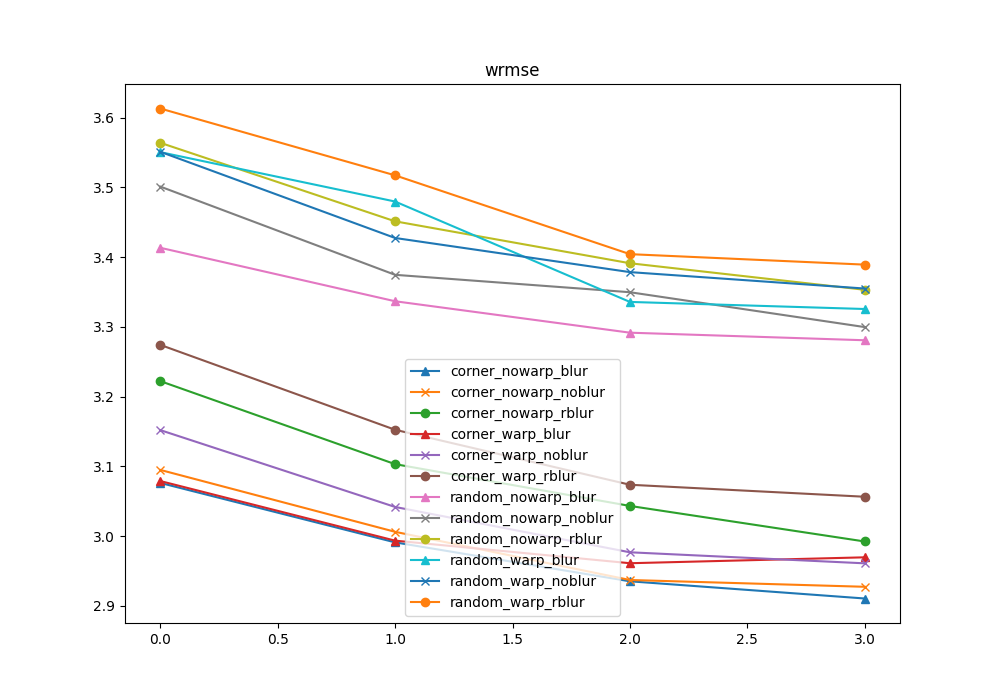
\includegraphics[width=\textwidth]{figs/wrmse}
        \end{subfigure}
        \hspace{0cm}
        \begin{subfigure}{0.6\textwidth}
            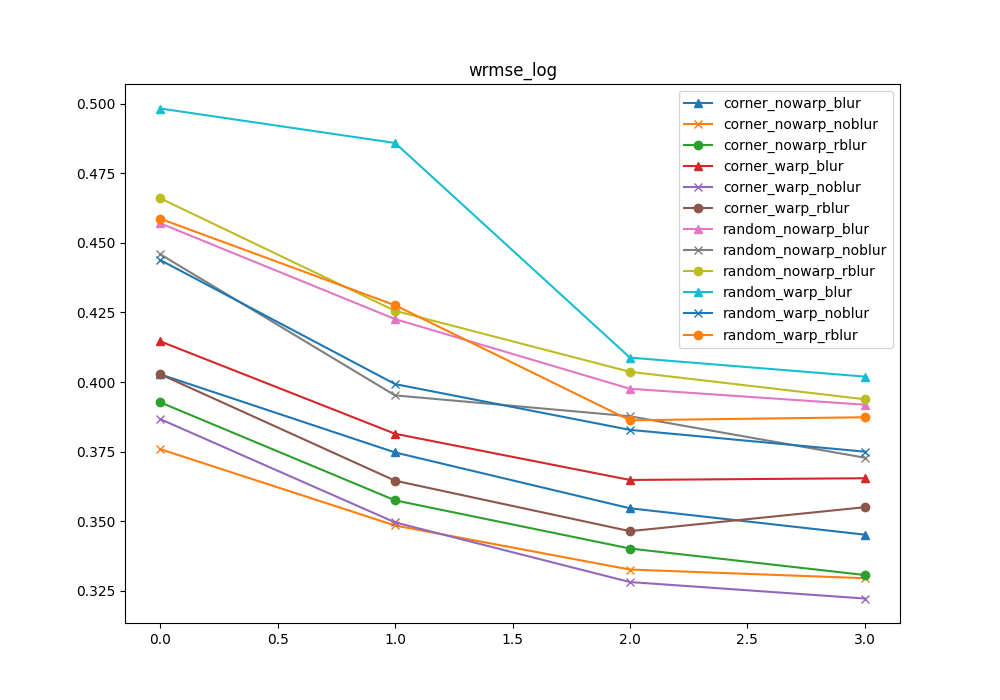
\includegraphics[width=\textwidth]{figs/wrmse_log}
        \end{subfigure}
        \hspace{0cm}
        \begin{subfigure}{0.6\textwidth}
            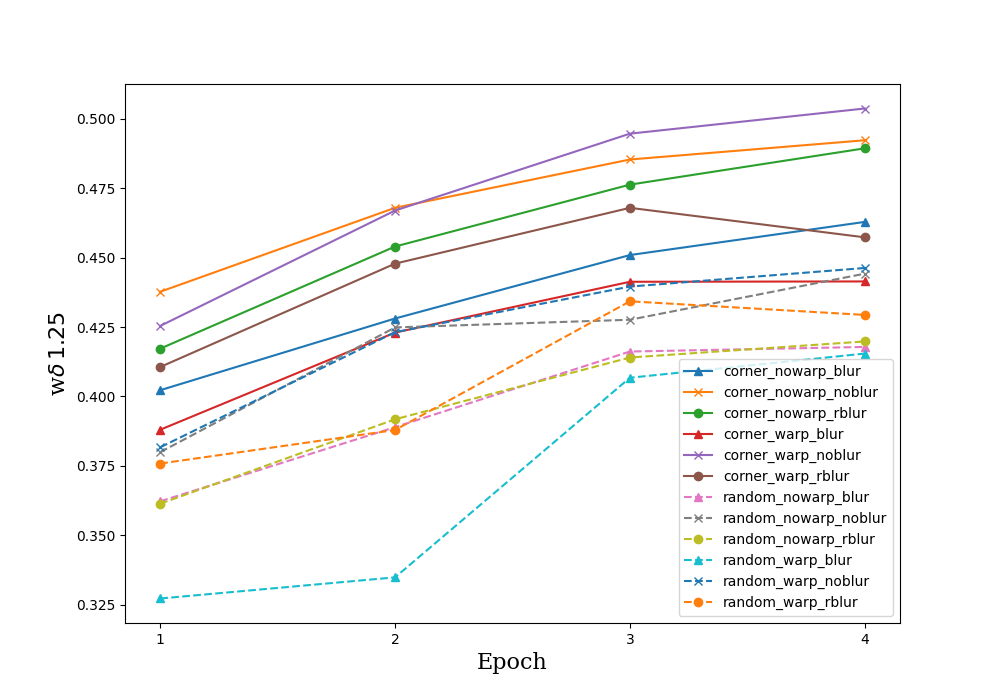
\includegraphics[width=\textwidth]{figs/wa1}
        \end{subfigure}
        \hspace{0cm}
        \begin{subfigure}{0.6\textwidth}
            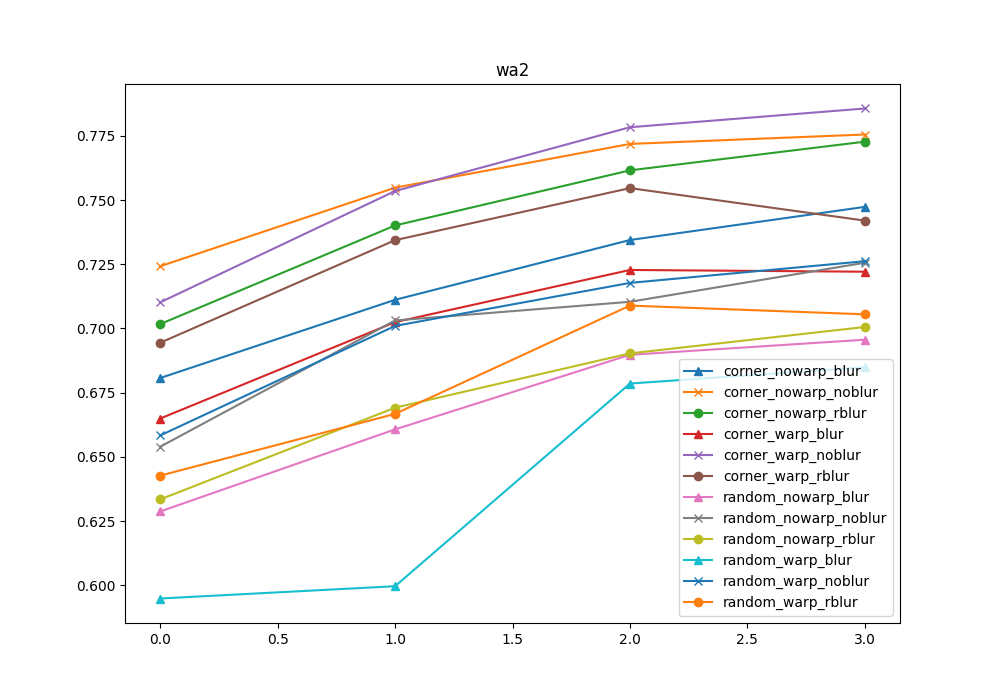
\includegraphics[width=\textwidth]{figs/wa2}
        \end{subfigure}
        \hspace{0cm}

        \begin{subfigure}{0.6\textwidth}
            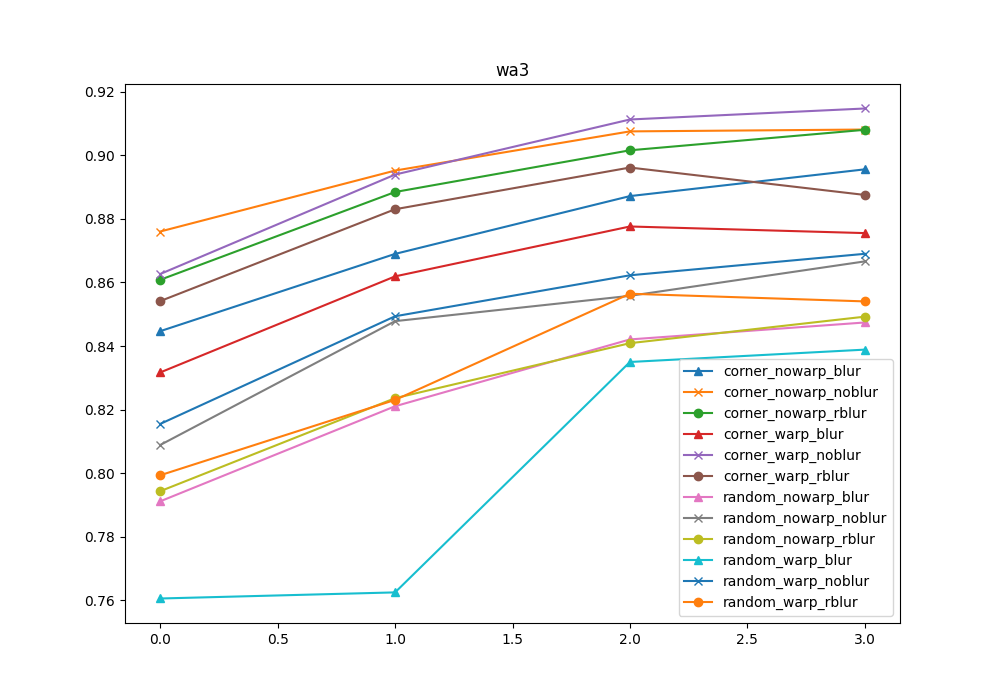
\includegraphics[width=\textwidth]{figs/wa3}
        \end{subfigure}
    \end{adjustwidth}
    \caption{
        \textbf{Weighted} metrics computed during the validation phase.
        \label{fig:Wvalidation}
    }
\end{figure}

\section{Discussion}
\label{sec:discussion}

All the trained models were tested on a held-out subset of the KITTI defined by the Eigen split.
All the numerical results obtained are reported in tables~\ref{t:results} and~\ref{t:weighted_results}.
The effect of each of the three options are now discussed: sampling strategy, warping and blurring.
These options are used both for training and evaluation.
Each of them defines a different learning problem with a different data distribution.
Single image depth estimation (SIDE) can be performed by fusing the predictions produced by each of the proposed learning setups.
To this extent, picking the options that maximize the performances allows for a better overall SIDE.
Results must be interpreted keeping this in mind.

\paragraph{Effect of sampling strategy.}
It is evident that the corner sampling defines a learning problem on which the network performs better.
This was also notable in the validation graphs and is true for all metrics without exceptions.
In~\cite{BoostingDepth} was observed that pretrained SIDE models perform better on image regions with a certain edge density.
Here it is proved that defining the SIDE problem on better-behaved image regions results in a simpler learning problem for the model.
This is likely due to a correlation of corners with visual depth cues.

\paragraph{Effect of warping.}
Warping seems to mildly simplify the learning problem too.
In the non-weighted metrics table~\ref{t:results}, while some best or second-to-best results are associated to the presence of warping, there isn't an overall performance improvement.
Instead, in table~\ref{t:wighted_results}, warping is present in all best performing models except for one problem setting.
Since the training loss was itself weighted, the weighted metrics are the reference for these experiments.
Hence, it can be concluded that: geometrically correcting the patches by appropriately warping them lead to little improvements.
Further investigation is needed for assessing the real utility of this additional preprocessing.
In any case, it must be noted that the warping procedure itself introduces some interpolation error that could have influenced results.
There could be better warping procedures that are less affected by this.

\paragraph{Effect of blurring.}
The radial blurring options never appears in the best performing models.
Radial blurring actually degrades the performance of the model.
The explanation for this has to be found in the model architecture.
In the convolutional layers of the network, kernel computations are performed in the same way all over the image.
Radially blurring the input creates differences in the central part of it from the borders.
It is realistic to assume that blurred and sharp regions need \textit{different} convolution kernels for capturing their features.
This creates a competition within the input image itself which leads to a degradation of performances.

I experimented also with a uniform blur of the whole input image.
Uniformly blurring the image improves non-weighted metrics as it probably acts as a regularization, though it degrades the weighted one since information related to the most weighted patch region is lost in the blurring.

This proves that the blurring can be beneficial to the learning problem as long as the hypothesis space is adjusted accordingly.

\begin{table}
    \begin{adjustwidth}{-0.2\textwidth}{-0.2\textwidth}
        \centering
    \begin{tabular}{c|c|c|c|c|c|c|c|c|c}
        \emph{Sampling} & \emph{Warp} & \emph{Blur} & \emph{MARE} & \emph{MSRE} & \emph{RMSE} & \emph{RMSEL} & \emph{$\delta \, 1.25$} & \emph{$\delta \, 1.25^{2}$} & \emph{$\delta \, 1.25^{3}$} \\
        \hline
        Random & No  & No      &            0.427  &            7.212  &            13.113  &            0.742  &            0.281  &            0.471  &            0.603  \\
        Random & No  & Radial  &            0.444  &            7.669  &            13.536  &            0.781  &            0.249  &            0.446  &            0.577  \\
        Random & No  & Uniform &            0.427  &            7.168  &            13.037  &            0.725  &            0.289  &            0.478  &            0.609  \\
        Random & Yes & No      &            0.425  &            7.480  &            13.581  &            0.746  &            0.285  &            0.471  &            0.599  \\
        Random & Yes & Radial  &            0.438  &            7.685  &            13.794  &            0.771  &            0.263  &            0.452  &            0.580  \\
        Random & Yes & Uniform &            0.424  &            7.205  &            13.363  &            0.706  &            0.274  &            0.474  &            0.613  \\
        Corner & No  & No      &    \textbf{0.387} & \underline{5.109} & \underline{10.674} &            0.631  & \underline{0.306} &            0.532  &            0.688  \\
        Corner & No  & Radial  &            0.410  &            5.523  &            11.091  &            0.679  &            0.280  &            0.494  &            0.653  \\
        Corner & No  & Uniform & \underline{0.389} &    \textbf{4.915} &    \textbf{10.461} &    \textbf{0.601} &    \textbf{0.316} &    \textbf{0.556} &    \textbf{0.718} \\
        Corner & Yes & No      &    \textbf{0.387} &            5.208  &            10.925  &            0.631  & \underline{0.306} &            0.532  &            0.689  \\
        Corner & Yes & Radial  &            0.415  &            5.857  &            11.629  &            0.707  &            0.257  &            0.464  &            0.624  \\
        Corner & Yes & Uniform &    \textbf{0.387} &            5.261  &            11.081  & \underline{0.615} &            0.302  & \underline{0.535} & \underline{0.697} \\
    \end{tabular}
    \end{adjustwidth}
    \caption{
        Performances on the test set.
        Bold numbers are the minimum (for error metrics) or the maximum (for accuracy metrics) in the column.
        Underlined numbers are the second-best result in that same column.
        \label{t:results}
    }
\end{table}

\begin{table}
    \begin{adjustwidth}{-0.2\textwidth}{-0.2\textwidth}
    \centering
    \begin{tabular}{c|c|c|c|c|c|c|c|c|c}
        \emph{Sampling} & \emph{Warp} & \emph{Blur} & \emph{wMARE} & \emph{wMSRE} & \emph{wRMSE} & \emph{wRMSEL} & \emph{w$\delta \, 1.25$} & \emph{w$\delta \, 1.25^{2}$} & \emph{w$\delta \, 1.25^{3}$} \\
        \hline
        Random & No  & No      &             0.323  &            5.024  &            3.364  &            0.389  &            0.423  &            0.699  &            0.849  \\
        Random & No  & Radial  &             0.332  &            5.361  &            3.420  &            0.412  &            0.398  &            0.676  &            0.830  \\
        Random & No  & Uniform &             0.344  &            5.498  &            3.351  &            0.415  &            0.391  &            0.664  &            0.824  \\
        Random & Yes & No      &             0.320  &            5.314  &            3.424  &            0.398  &            0.420  &            0.694  &            0.843  \\
        Random & Yes & Radial  &             0.331  &            5.541  &            3.463  &            0.410  &            0.402  &            0.674  &            0.828  \\
        Random & Yes & Uniform &             0.351  &            5.928  &            3.403  &            0.426  &            0.385  &            0.652  &            0.813  \\
        Corner & No  & No      &             0.299  &            3.921  & \underline{3.045} & \underline{0.352} & \underline{0.461} & \underline{0.743} & \underline{0.889} \\
        Corner & No  & Radial  &             0.317  & \underline{4.090} &            3.117  &            0.356  &            0.453  &            0.737  &            0.886  \\
        Corner & No  & Uniform &             0.336  &            4.480  &    \textbf{3.030} &            0.373  &            0.425  &            0.711  &            0.871  \\
        Corner & Yes & No      &     \textbf{0.301} &    \textbf{4.059} &            3.088  &    \textbf{0.349} &    \textbf{0.465} &    \textbf{0.746} &    \textbf{0.893} \\
        Corner & Yes & Radial  &  \underline{0.310} &            4.560  &            3.187  &            0.387  &            0.416  &            0.697  &            0.857  \\
        Corner & Yes & Uniform &             0.337  &            5.026  &            3.105  &            0.404  &            0.392  &            0.670  &            0.841  \\
    \end{tabular}
    \end{adjustwidth}
    \caption{
        Performances on the test set of the \textbf{weighted} metrics.
        Bold numbers are the minimum (for error metrics) or the maximum (for accuracy metrics) in the column.
        Underlined numbers are the second-best result in that same column.
        \label{t:weighted_results}
    }
\end{table}